\chapter{Stand der Technik}\label{ch:StandDerTechnik}
% Auch "Stand der Forschung" oder "Stand der Praxis"

% Bezogen auf die eigenen Zielsetzungen und Fragestellungen soll aufgezeigt werden, wie andere
% dieses oder ähnliche Probleme gelöst haben. Worauf können Sie aufbauen, was müssen Sie neu
% angehen? Wodurch unterscheidet sich Ihre Lösung von anderen Lösungen? Für wissenschaftlich
% orientierte Arbeiten sei hier explizit auf (Balzert, S. 66 ff) verwiesen.

% TODO Historie des betroffenen Feld

\section{Technologische Grundlagen}
% TODO Wichtige technologischen Grundlagen / Wissenswertes

\subsection{P2P Netzwerke}

Scope: Nur I2P

\subsection{Performance / Bandwidth / Latency}

\subsection{I2P}

I2P ist ein \glsname{p2p}-Netzwerk.

\begin{itemize}
    \item Unabhängiges Netzwerk
    \item Low-Latency
    \item \glstext{e2e}
\end{itemize}

\cite{astolfi_i2p_2015}
\cite{astolfi_i2p_nodate}

\cite{timpanaro_birds_2012}

\cite{timpanaro_evaluation_2015}

A scaleable framework for anonymous communication
\cite{noauthor_i2p_nodate-8}


\cite{hoang_measuring_2019}
\cite{hoang_empirical_2018}

\cite{de_boer_invisible_2019}

\cite{zantout_i2p_2011}

Latency vs Tor Usability Bandwith and Latency Comparision
\cite{ehlert_i2p_2021}

\subsection{Wie I2P funktioniert}

\begin{itemize}
    \item Jeder Knoten leitet auch traffic für das Netzwerk weiter
    \item Jeder Knoten kann die länge 
\end{itemize}

\section{Technische Konzepte}
\label{sec:technischeKonzepte}
% TODO Konzepte in diesem Feld welche für den Leser relevant sind

\subsection{Tunnels}

Jeder I2P-Router kann eine beliebige Anzahl Inbound- und Outbound Tunnels erstellen.
Wobei die Inbound Tunnels zum Empfang und die Outbound-Tunnels zum Versand dienen.

%TODO: inbound outbound nicht verwechseln

Jedes Tunnel hat eine Länge.
Diese gibt an durch wie viele Knoten eine Nachricht, die durch das Tunnel verschickt wird, geroutet wird.
Für jeden Hop im Tunnel wird die Nachricht eine zusätzliche Verschlüsselungsschicht eingehüllt. (vgl. Onion Routing)
Somit wissen die Router jeweils nur Bescheid von welchem anderen Router sie eine Nachricht erhalten haben und an welchen Router die Nachricht weitergeleitet werden soll.
Ein Roter im Tunnel weiss also schlussendlich nie von wem an wen eine Nachricht verschickt wurde.

Die Länge eines Tunnels kann auch \lstinline|0| betragen.
In diesem Fall wird eine Nachricht die durch das Tunnel verschickt wird, durch keine weitere Knoten geroutet.

Hierbei kann jeder Knoten selber festlegen wie lange diese Tunnels sind.

Je Länger ein Tunnel ist, desto mehr Anonymität bietet dieser.
Jedoch geht dies auf Kosten der Latenz aufgrund der zusätzlichen Hops.

Tunnels Configuration
\cite{noauthor_i2p_nodate-3}

\begin{itemize}
    \item Jeder Knoten kann die länge seiner Tunnel selber bestimmen. (Standardwert 3)
    \item Mehrere Verschlüsslungslayer je nach Tunnellänge (vgl. Onion-Routing)
\end{itemize}

\subsection{Garlic-Routing}

Im Gegensatz zum \glsname{tor}-Netzwerk setzt

\begin{itemize}
    \item
\end{itemize}

\subsection{NetDB}

\subsection{Reseeding}

Seeding etc.

Reseed Access
\cite{noauthor_i2p_nodate-7}


\section{Technische Konzepte}
\label{sec:technischeKonzepte}
% TODO Konzepte in diesem Feld welche für den Leser relevant sind

\subsection{Das Anonymitätstrilemma}\label{sec:anonymitytrilemma}

Beim Design eines anonymen Kommunikationsprotokoll gibt es gründsätzliche Einschränkungen. Es gilt die folgenden drei Aspekte abzuwägen:

\begin{itemize}
    \item Hoher Anonymiätsgrad von Sender und Empfänger einer Nachricht
    \item Tiefer Netzwerkbandbreiten Overhead
    \item Tiefer Latenz Overhead
\end{itemize}

Dabei ist es nicht möglich ein Protokoll zu designen welches alle diese drei Aspekte komplett erfüllt.
Es muss entschieden werden, welche zwei Aspekte wichtiger sind (siehe auch die Abbildung~\fullref{fig:anonimitytrilemma}). \parencite{das_anonymity_2018}

\begin{figure*}[h]
    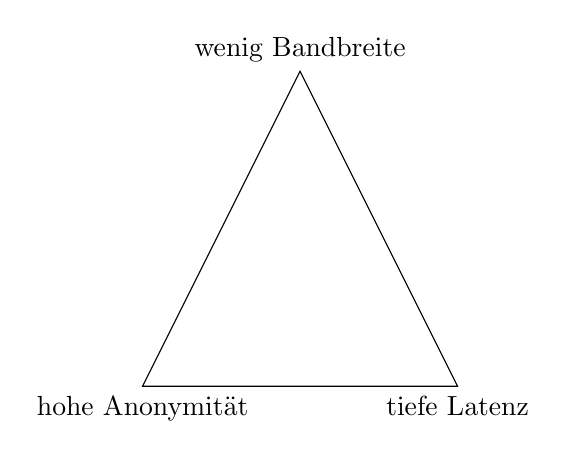
\begin{tikzpicture}
      \draw (0,0) node[anchor=north]{hohe Anonymität}
        -- (4,0) node[anchor=north]{tiefe Latenz}
        -- (2,4) node[anchor=south]{wenig Bandbreite}
        -- cycle;
    \end{tikzpicture}
    \caption{Das Anonymitätstrilemma}\label{fig:anonimitytrilemma}
\end{figure*}

Zum Beispiel wenn ein hoher Anonymitätsgrad erwünscht ist, kann dies nur erreicht werden mit entweder mehr Netzwerkbandbreiten-Overhead oder mehr Latenz-Overhead.


\section{Stand im Bezug auf eigenes Projekt}
% TODO Welche Forschung wurde in jüngster Zeit gemacht welche relevant für das eigene Projekt sind

Usability Inspection of Anonmity Networks
(\cite{abou-tair_usability_2009})

Usability Tetsts

(\cite{schomburg_anonymity_2009})

Evaluation of Anonymity Networks
(\cite{timpanaro_evaluation_2015})

\subsection{Performance}


Performance improvement using SSL IN I2P
\cite{vashi_performance_2015}

Performance I2P Webseite
\cite{noauthor_performance_nodate}

Performance History I2P Webseite
\cite{noauthor_performance_nodate-1}

Auf der Webseite von I2P auf der Seite ''Future Performance Improvements'' sind zudem zukünftige Performance Verbesserungsmöglichkeiten aufgelistet.
\cite{noauthor_future_nodate}
On I2P's website the page 

Improving I2P (2012)
\cite{timpanaro_improving_2012}


\subsection{I2P-Testnetzwerke}

\subsection{Metriken zur Messung}

Towards Measuring on the I2P Netzwork
\cite{wang_towards_2013}

\begin{itemize}
    \item Latenzmessung (abschicken/empfangen (Laport-Zeitstempel im schlimmsten fall))
    \item Messung der Bandbreite (ab welchem Layer)
    \item Ressourcenauslastung
\end{itemize}

\cite{timpanaro_monitoring_nodate}

\subsection{Testen im öffentlichen I2P Netzwerk}

\begin{itemize}
    \item family tag \cite{noauthor_family_nodate}
    \item verfälscht resultate
    \item deshalb isolieren
    \item öffentliche Metriken  I2P Metrics: \cite{noauthor_i2p_nodate-4}
    \item Netzwerk ist klein (deshalb braucht es so ein beweis wie hier)
\end{itemize}
